\chapter{Benchmarking Results}\label{chapter:analysis}

The results presented in this chapter have been calculated on a x64 architecture (Intel(R) Core(TM) i5-6200U CPU @ 2.30GHz) running Ubuntu 20.04.1 LTS. The installed docker version was 19.03.8. The benchmarking suite was initialized to run callgrind and massif 100 times, respectively (e.g. $N=100$). All values presented in this chapter are averages over $N=100$ samples. Additionally, all graphs contain the standard derivation (If no standard derivation can be observed in a particular graph, the value is zero or too small to be drawn). The exact values and the identified execution hotspots for all implementations instantiated respectively with all parameter sets (see \autoref{sec:included_implementations}) can be found in addenda \ref{app:detailed_benchmarks}. The efficiency in this chapter is quantified by the peak memory consumption and by the absolute instruction count measured by the benchmarking suite (details in \autoref{chapter:benchmarking_suite}). \\
The graphs below use the following terminology:
Assume Alice (A) and Bob (B) want to establish a shared secret using a \gls{SIDH} key exchange.
\begin{itemize}
\item \textit{KeygenA} describes the key generation (public and private key) of Alice.
\item \textit{KeygenB} describes the key generation (public and private key) of Bob.
\item \textit{SecretA} describes the computation of the shared secret by Alice.
\item \textit{SecretB} describes the computation of the shared secret by Bob.
\end{itemize}
This chapter starts with a comparison between all \gls{SIDH} security levels in \autoref{sec:analysis_sidh_levels}. This demonstrates the performance differences of the available parameter sets. \\
A comparison among all available \gls{SIKE} implementations is given in \autoref{sec:analysis_sike}: This section  works out differences between \textit{reference}, \textit{generic optimized}, \textit{x\_64 optimized} and \textit{compressed} implementations of SIKE. Moreover, the previously mentioned similarities and differences between \gls{PQCrypto-SIDH} and \gls{SIKE} are investigated based on the measured benchmarking results. \\
In \autoref{sec:sike_vs_circl} the comparison between \gls{SIKE} and \gls{CIRCL} is drawn to identify the most performant SIDH key exchange implementation. This section also analyses the observed execution hotspots of both libraries.\\
Differences in terms of efficiency between modern state-of-the-art \gls{ECDH} and quantum-resistant \gls{SIDH} are pointed out in \autoref{sec:analysis_effiency_ecdh}. This section also highlights execution hotspots measured for \gls{ECDH}.\\
The chapter concludes with security considerations for all benchmarked implementations in terms of constant time cryptography and key size (\autoref{sec:analysis_security}). 

\section{Comparing \gls{SIDH} security levels}\label{sec:analysis_sidh_levels}

Before drawing any differences between libraries or implementations, this section considers the different parameter sets proposed in \parencite{sike2020spec}: \texttt{p434}, \texttt{p503}, \texttt{p610} and \texttt{p751}. All these parameters match a security level defined by \gls{NIST} (see \autoref{sidh_security} for details). This section makes use of the \texttt{SIKE\_x64} implementation to visualize the claimed resources of the different parameter sets. Additionally, this section also compares the currently deployed \gls{SIDH} parameters to classical elliptic curve cryptography parameters: \texttt{secp256}, \texttt{secp384} and \texttt{secp521}. Recall the security classes of all parameter sets:

\begin{table}[H]
	\centering
	\begin{tabular}{|K{4cm}|K{4cm}|K{4cm}|}
	\hline
	\rowcolor{lightgray!50}
	\bfseries\makecell{Security Level} & \bfseries\makecell{SIDH parameters} & \bfseries\makecell{ECDH parameters} \\
	\hline
	\makecell{\gls{NIST} level 1} & \makecell{p434} & \makecell{secp256} \\
	\hline
	\makecell{\gls{NIST} level 2} & \makecell{p503} & \makecell{-} \\
	\hline
	\makecell{\gls{NIST} level 3} & \makecell{p610} & \makecell{secp384} \\
	\hline
	\makecell{\gls{NIST} level 5} & \makecell{p751} & \makecell{secp521} \\
	\hline
	\end{tabular}
	\caption[NIST security levels with SIDH and ECDH parameters]{NIST security levels with SIDH and ECDH parameters.}
	\label{tab:benchmarks_Sike_x64}
\end{table}

\autoref{fig:results_all_curves} shows the absolute instruction counts for \texttt{SIKE\_x64} initialized with all available parameter sets. While \texttt{p434} executes 18 million instructions for \textit{KeygenA}, \texttt{p751} requires 67 million operations ($3.7$ times more). Roughly the same can be observed regarding \textit{KeygenB}, \textit{SecretA} and \textit{SecretB}. The other parameter sets \texttt{p503} and \texttt{p610} almost lie on a linear line between the highest and lowest security class. At the same time the \gls{ECDH} implementations are clearly faster while providing the same security levels: \texttt{Secp256} processes in total 1.7 million instructions while \texttt{p434} executes 69 million operations (40.6 times more) for a single \gls{SIDH} key exchange. \texttt{Secp384} (40 million) executes 4.3 times more instructions than \texttt{p610} (170 million) and \texttt{secp521} (96 million) executes 2.6 times more instructions than \texttt{p751} (253 million).\\
The measured peak memory consumption is for \texttt{p751} the highest ($13.3$ \gls{kB}) and for \texttt{p434} the lowest ($8.2$ \gls{kB}) among \gls{SIDH} parameters. Again, further parameter sets can be found in between of these boundary values (\autoref{fig:results_all_curves_mem}). Moreover, one can observe an increased memory consumption of \gls{ECDH} parameters: Compared to \texttt{p434}, the elliptic curve parameter set \texttt{secp256} demands 4 $kB$ more memory. \texttt{Secp384} and \texttt{secp521} allocate 3 $kB$ additionaly memory compared to their appropriate \gls{SIDH} parameters, respectively.\\\\
This analysis clearly demonstrates that an increased security level of \gls{SIDH} corresponds with a increased claim of resources. Whereas the difference in terms of memory consumption is relatively small, the execution times differ noticably: On average and compared to \texttt{p434} the parameter set
\begin{itemize}
\itemsep0em 
\item \texttt{p503} executes $1.4$ times more instructions
\item \texttt{p610} executes $2.5$ times more instructions
\item \texttt{p710} executes $3.7$ times more instructions
\end{itemize}
While the \gls{ECDH} parameter sets enable faster computation times for a single key exchange, they also suffer from an increased memory consumption. The reason for this might be a trade-off between execution time and memory consumption for implementing secure cryptography. Increased memory allocations for available \gls{SIDH} parameters might also need to be taken into account in future to further reduce execution times.

\begin{figure}[H]
  \centering
  \includegraphics[width=0.9\textwidth]{benchmarks/all_curves/SIKE_x64}
  \caption[Overall instructions for all parameter sets via \texttt{SIKE\_x64} compared to \texttt{ECDH}]
  {Overall instructions for \texttt{SIKE\_x64} initiated with all possible parameter sets compared to appropriate \texttt{ECDH} parameter sets.}
  \label{fig:results_all_curves}
\end{figure}

\begin{figure}[H]
  \centering
  \includegraphics[width=0.9\textwidth]{benchmarks/all_curves/SIKE_x64_mem}
  \caption[Maximum memory consumption for all parameter sets via \texttt{SIKE\_x64}  compared to \texttt{ECDH}]
  {Maximum memory consumption in kilobytes of \texttt{SIKE\_x64} initiated with all possible parameter sets compared to appropriate \texttt{ECDH} parameter sets.}
  \label{fig:results_all_curves_mem}
\end{figure}


\section{Comparing \gls{SIKE} implementations}\label{sec:analysis_sike}
Before the comparisons between the \gls{SIDH} libraries \textit{\gls{SIKE}} and \textit{\gls{CIRCL}} are drawn, the differences of available \textit{\gls{SIKE}} implementations are investigated. Besides a \textit{reference} implementation, the library provides \textit{generic optimized} and \textit{x64 optimized} variants. This section analyzes the differences between these \textit{optimized} implementations. Moreover,  \textit{compressed} versions for both \textit{optimized} variants are available. The performance differences between \textit{compressed} and \textit{non-compressed} versions are additionally emphasized in this section. Note that all \textit{compressed} versions of \gls{SIKE} also contain \textit{optimized} code. Their key sizes, however, are reduced compared to non-compressed variants. Since the previous section investigated differences between \gls{SIDH} parameter sets this section only considers \texttt{p434}.


\subsubsection{Reference implementation}
The \texttt{SIKE\_Reference} implementation is with 11.2 \gls{kB} allocated memory close to the average ($\sim$ 12.7 \gls{kB}) of all \gls{SIKE} implementations (see \autoref{fig:results_sike_mem}). Regarding the execution times for key generation in \autoref{fig:results_sike}, the reference implementation is by far the slowest variant: More than 2.3 billion ($2.300.000.000$) instructions were measured in order to generate Bobs key pair. This is slower by factor 100 compared to \texttt{SIKE\_x64}. As the name suggests, this reference implementation must be seen as a proof-of-concept. Thus, performance criteria are no requirements for this implementation, which is confirmed by the observed benchmarking results.

\subsubsection{Optimized implementations}
\gls{SIKE} provides two \textit{optimized} implementations: \texttt{SIKE\_generic} and \texttt{SIKE\_x64}. The benchmarks in \autoref{fig:results_sike} show a significant speed up of \texttt{SIKE\_x64} compared to \texttt{SIKE\_generic}. Key generation for Alice and Bob is 10.8 times faster and secret generation about 11 times. At the same time \texttt{SIKE\_generic} allocates 7.7 \gls{kB} memory, which is 0.5 \gls{kB} less than the x64 optimized variant (\autoref{fig:results_sike_mem}). Thus, the increased speed involves the allocation of more memory -- a time-memory trade-off \parencite{1056220}.

\subsubsection{Compressed implementations}
\autoref{fig:results_sike} clearly shows a difference between \textit{optimized} and \textit{compressed} versions of \gls{SIKE} in terms of absolute instructions. Compressed versions roughly claim twice as much operations ($\sim$ 500 million for \texttt{SIKE\_Generic\_Compressed} and $\sim$ 45 million \texttt{SIKE\_x64\_Compressed}) to generate a key pair as non-compressed variants ($\sim$ 200 million for \texttt{SIKE\_Generic} and $\sim$ 19 million \texttt{SIKE\_x64}). Additionally, the generation of the shared secret  using compressed implementations is slightly slower.\\
Besides execution times, \autoref{fig:results_sike_mem} also compares the memory consumption. As stated by the authors of \gls{SIKE}, compressed variants allocate more memory~\parencite{sike2020spec}: The peak memory allocation is with 17 kilobytes (\texttt{SIKE\_Generic\_Compressed}) and 19.2 kilobytes (\texttt{SIKE\_x64\_Compressed}) twice as high as for the non-compressed versions.\\
The comparison between all \gls{SIKE} implementations showed that \textit{optimized} versions have decreased instructions counts as well as decreased memory consumptions compared to \textit{compressed} implementations. Roughly speaking, \textit{compressed} versions demand twice as much resources than \textit{optimized} variants, while decreasing the effective key sizes (see \autoref{sec:analysis_security_keys} for details).



\begin{figure}[H]
  \centering
  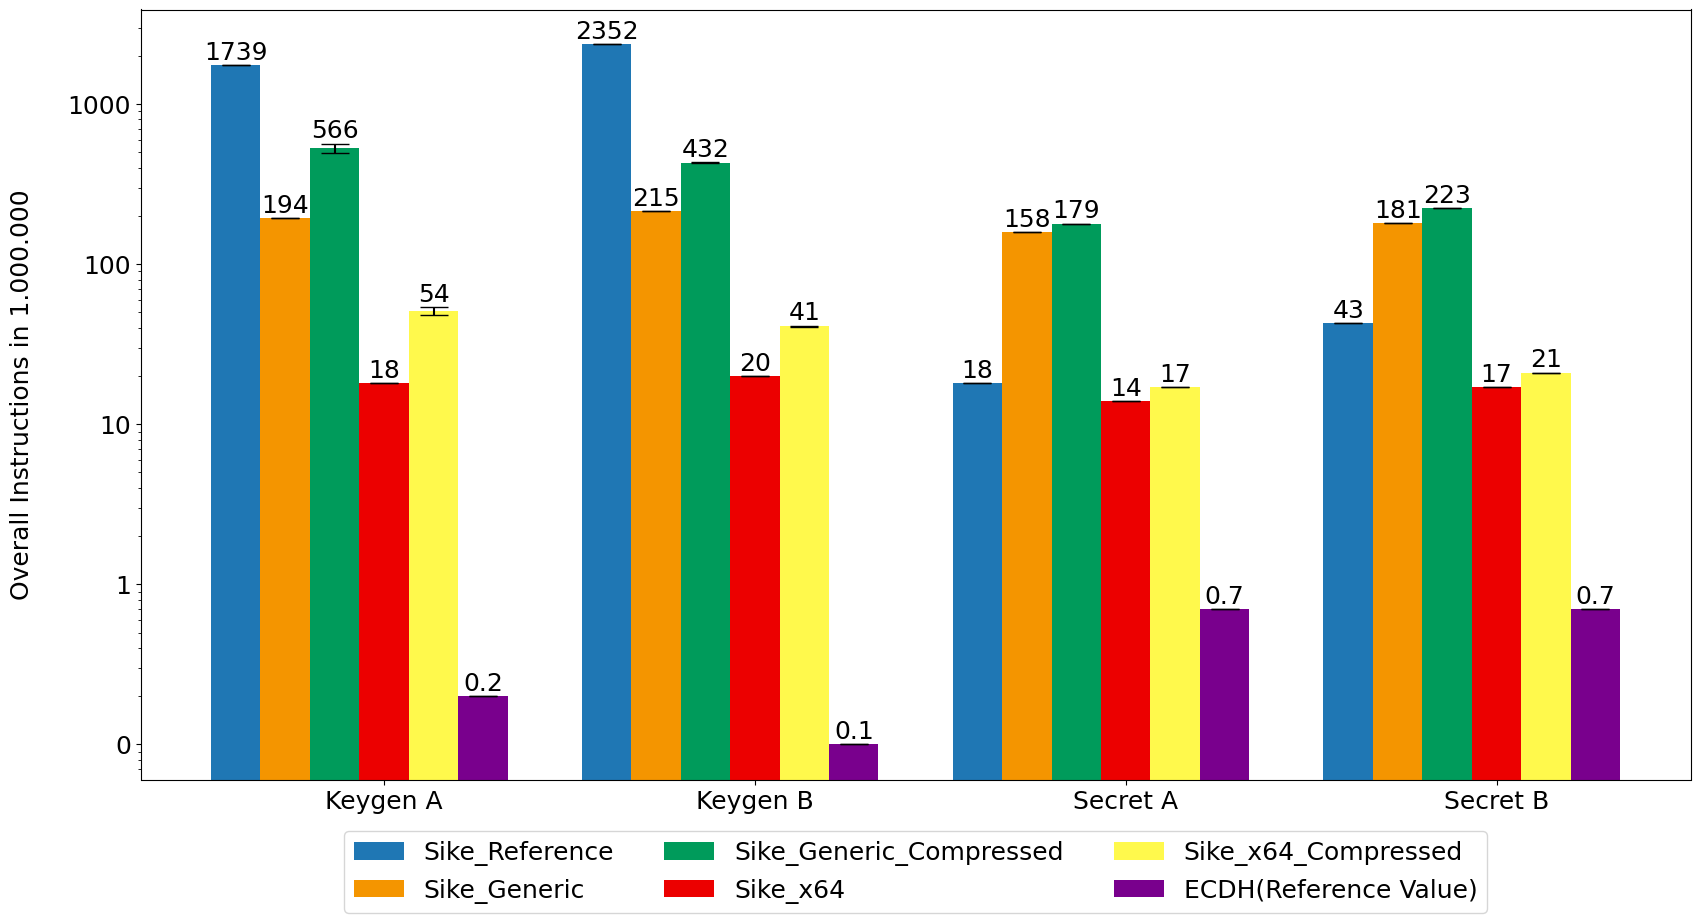
\includegraphics[width=1\textwidth]{benchmarks/sike/sike}
  \caption[Overall instructions \gls{SIKE}]
  {Overall instructions for all \gls{SIKE} implementations initialized with \texttt{p434}. \gls{ECDH} is shown as reference value using parameter \texttt{secp256}.}
  \label{fig:results_sike}
\end{figure}

\begin{figure}[H]
  \centering
  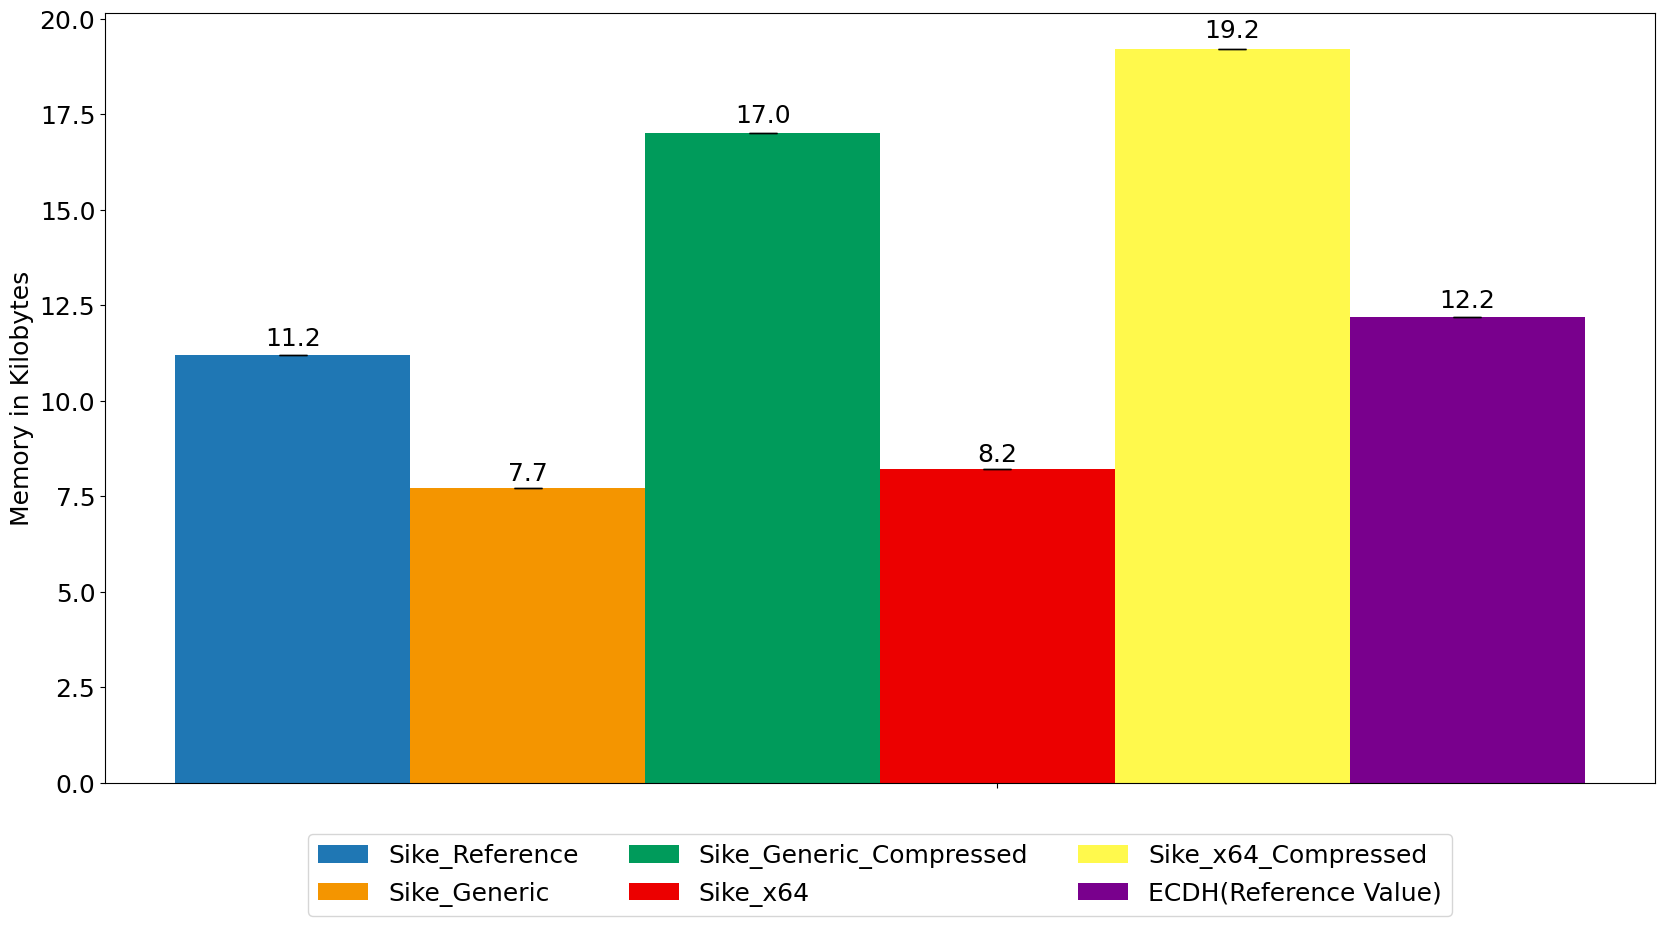
\includegraphics[width=1\textwidth]{benchmarks/sike/sike_mem}
  \caption[Maximum memory consumption \gls{SIKE}]
  {Maximum memory consumption in kilobytes or all \gls{SIKE} implementations initialized with \texttt{p434}. \gls{ECDH} is shown as reference value using parameter \texttt{secp256}.}
  \label{fig:results_sike_mem}
\end{figure}

\subsection{\gls{PQCrypto-SIDH} vs. \gls{SIKE}}

This section describes the similarities and differences between \gls{PQCrypto-SIDH} and \gls{SIKE}. Note, that the \gls{SIKE} team uses the Microsoft Github repository of \gls{PQCrypto-SIDH} to create their \gls{NIST} submissions (see \autoref{existing:sike_vs_pqcrypto} for details). At the same time the libraries reveal considerable differences when analyzing their \textit{compressed} versions. Compressed implementations of \gls{SIDH} promise shortened key size compared to non-compressed versions, however, this leads to increased execution times and memory allocations. 
\\\\
\subsubsection{Optimized implementations}

\subsubsection{Compressed implementations}
\autoref{fig:results_comp_434} shows the execution time benchmarks for the compressed variants of \gls{PQCrypto-SIDH} and \gls{SIKE} initiated with \texttt{p434}. Naturally, the x64 optimized code is faster than the generic optimization. The Microsoft implementations executed less operations than \gls{SIKE}: Regarding key generation, \textit{SIKE\_Generic\_Compressed} performed on average $38$\% more instructions than \textit{Microsoft\_Generic\_Compressed}. \textit{SIKE\_x64\_Compressed} performed on average $45$\% more instructions than \textit{Microsoft\_x64\_Compressed}. The generation of the secret key only shows slight differences between \gls{SIKE} and Microsoft, however Microsoft remains the fastest. The trend of this analysis also applies to improved security classes, e.g to parameter \textit{p751} (see \autoref{fig:results_comp_751})
\\
The following evaluation of the allocated memory is surprising (\autoref{fig:results_comp_434_mem}): The Microsoft implementations occupy three times more memory than \gls{SIKE} when initiated with \textit{p434}. This gap rises strongly when increasing the security class to \textit{p751} (\autoref{fig:results_comp_751_mem}), where the the \textit{ \gls{PQCrypto-SIDH}} library of Microsoft allocates almost seven times more memory.
\\\\
While the benchmarks for the compressed Microsoft implementations show faster execution times, the overhead of allocated memory compared to \gls{SIKE} is enormous.

\begin{figure}[H]
  \centering
  \includegraphics[width=1\textwidth]{benchmarks/MicrosoftSike/compressed/434}
  \caption[Overall instructions compressed p434]
  {Overall instructions for compressed \gls{SIDH} parameter \texttt{p434}.}
  \label{fig:results_comp_434}
\end{figure}

\begin{figure}[H]
  \centering
  \includegraphics[width=1\textwidth]{benchmarks/MicrosoftSike/compressed/434_mem}
  \caption[Maximum memory consumption compressed p434]
  {Maximum memory consumption in kilobytes for compressed \gls{SIDH} parameter \texttt{p434}.}
  \label{fig:results_comp_434_mem}
\end{figure}

\begin{figure}[H]
  \centering
  \includegraphics[width=1\textwidth]{benchmarks/MicrosoftSike/compressed/751}
  \caption[Overall instructions compressed p751]
  {Overall instructions for compressed \gls{SIDH} parameter \texttt{p751}.}
  \label{fig:results_comp_751}
\end{figure}

\begin{figure}[H]
  \centering
  \includegraphics[width=1\textwidth]{benchmarks/MicrosoftSike/compressed/751_mem}
  \caption[Maximum memory consumption compressed p751]
  {Maximum memory consumption in kilobytes for compressed \gls{SIDH} parameter \texttt{p751}.}
  \label{fig:results_comp_751_mem}
\end{figure}

\section{Comparing \gls{SIKE} and \gls{CIRCL}} \label{sec:sike_vs_circl}


\subsection{Comparing optimized implementations}\label{sec:analysis_optimized}
This subsection firstly compares generic optimized \gls{SIDH} variants before x64 optimized implementations are analyzed.
\subsubsection{Generic optimized implementations}\label{sec:analysis_generic}
Generic optimized implementations contain generally optimized code for various hardware platforms. However, no hardware specific instructions can be exploited in these versions. The benchmarking suite currently supports \footnote{Although \gls{CIRCL} states to offer a generic optimized implementation\parencite{circl2020github}, this version could not be compiled.}:
\begin{enumerate}
\item \textit{SIKE\_Generic}
\item \textit{Microsoft\_Generic}
\end{enumerate}
\autoref{fig:results_opt_434} shows the benchmarks for execution time of all optimized variants initiated with \texttt{p434}. For this section, however, only \textit{SIKE\_Generic} and \textit{Microsoft\_Generic} are taken into account. In all four steps of the \gls{SIDH} key exchange, the benchmarked values for both implementations look almost the same. However, when considering exact measurements from  \ref{app:detailed_benchmarks}, one can observe that \textit{SIKE\_Generic} executes constantly half a million operations less than \textit{Microsoft\_Generic} (this holds for all four categories: Keygen A, Keygen B, Secret A and Secret B). While this sounds significant, the relative difference is actually less than $0.01$\%. While the absolute gap further increases, when higher security classes are analyzed (about three million operations constant difference for \texttt{p751}), the relative disparity stays below $0.01$\%.
\\\\
Peak memory consumptions for parameter \textit{p434} are visualized in  \autoref{fig:results_opt_434_mem}. As in terms of execution time, memory allocation numbers between \textit{SIKE\_Generic} and \textit{Microsoft\_Generic} hardly differ: The \gls{SIKE} version occupies $0.3$ \gls{kB} less memory for \textit{p434} and $0.7$ \gls{kB} less than for \textit{p751}. Overall, the relative difference regarding memory consumption is about $5$\%.
\\\\
Although both implementations hardly differ in their performance benchmarks, one can state that \textit{SIKE\_Generic} demands less resources (executed instructions and memory) than \textit{Microsoft\_Generic}. This disparity, however, is marginal.


\subsubsection{x64 optimized implementations}
\label{sec:analysis_x64}
X64 optimized implementations exploit AMD64 specific hardware operations to improve performance on these machines. The benchmarking suite currently supports the following x64 optimized variants:
\begin{enumerate}
\item \textit{SIKE\_x64}
\item \textit{Microsoft\_x64}
\item \textit{\gls{CIRCL}\_x64}
\end{enumerate}
\autoref{fig:results_opt_434} shows the execution time benchmarks for all optimized variants initiated with \texttt{p434}. For this section, however, only \textit{SIKE\_x64}, \textit{Microsoft\_x64} and \textit{\gls{CIRCL}\_x64} are taken into account. In all four categories listed in the graph \textit{Microsoft\_x64}  is the fastest implementation. \textit{SIKE\_x64} is slightly slower executing about two million instructions more in each category. This corresponds to a relative difference of about $10$\%. The most expensive implementation in terms of performed operations is \textit{\gls{CIRCL}\_x64}: $40$\% more operations are needed in each step of the \gls{SIDH} key exchange compared to the fastest variant \textit{Microsoft\_x64}.
\\
\autoref{fig:results_opt_751} compares the implementations initiated with \textit{p751} - matching the highest \gls{NIST} security level 5. \textit{Microsoft\_x64} stays the fastest version while the relative differences to \textit{SIKE\_x64} ($5$\%) and \textit{\gls{CIRCL}\_x64} ($30$\%) decrease.
\\\\
In order to compare the memory consumption of the x64 optimized implementations, consider \autoref{fig:results_opt_434_mem}. The memory benchmarks of \textit{SIKE\_x64} ($8.2$ \gls{kB}) and \textit{Microsoft\_x64} ($8.9$ \gls{kB}) hardly differ, whereas \textit{\gls{CIRCL}\_x64} has a peak allocation of $24.7$ \gls{kB} for a single \gls{SIDH} key exchange. This is by factor 2.5 greater compared to the others. However, \autoref{fig:results_opt_751_mem} reveals that the memory consumption for \textit{\gls{CIRCL}\_x64} does barely change for higher security classes. Nevertheless,  \textit{\gls{CIRCL}\_x64} has the most intense memory consumption of all x64 optimized implementations and \textit{Microsoft\_x64} allocates roughly about $10$\% more memory than \textit{SIKE\_x64} (this holds respectively for all security classes) .
\\\\
The fastest x64 optimized \gls{SIDH} key exchange is performed by \textit{Microsoft\_x64}. \textit{SIKE\_x64} is slightly slower but allocates less memory than \textit{Microsoft\_x64}. The most resources are consumed by \textit{\gls{CIRCL}\_x64} (instruction count and memory allocations).

\begin{figure}[H]
  \centering
  \includegraphics[width=1\textwidth]{benchmarks/optimized/434}
  \caption[Overall instructions p434]
  {Overall instructions for \gls{SIDH} parameter \texttt{p434} compared to \gls{ECDH} via \texttt{secp256r1}.}
  \label{fig:results_opt_434}
\end{figure}

\begin{figure}[H]
  \centering
  \includegraphics[width=1\textwidth]{benchmarks/optimized/434_mem}
  \caption[Maximum memory consumption p434]
  {Maximum memory consumption in kilobytes for \gls{SIDH} parameter \texttt{p434} compared to \gls{ECDH} via \texttt{secp256r1}.}
  \label{fig:results_opt_434_mem}
\end{figure}

\begin{figure}[H]
  \centering
  \includegraphics[width=1\textwidth]{benchmarks/optimized/751}
  \caption[Overall instructions p751]
  {Overall instructions for \gls{SIDH} parameter \texttt{p751} compared to \gls{ECDH} via \texttt{secp521r1}.}
  \label{fig:results_opt_751}
\end{figure}

\begin{figure}[H]
  \centering
  \includegraphics[width=1\textwidth]{benchmarks/optimized/751_mem}
  \caption[Maximum memory consumption 751]
  {Maximum memory consumption in kilobytes for \gls{SIDH} parameter \texttt{p751} compared to \gls{ECDH} via \texttt{secp521r1}.}
  \label{fig:results_opt_751_mem}
\end{figure}

\subsection{Analysis of execution hotspots}\label{sec:analysis_sidh_hotspots}
Besides detailed benchmarks, addenda \ref{app:detailed_benchmarks} also lists the execution hotspots of each implementation initialized with different parameters. The following description of these hotspots reveals potentials to further improve performance of \gls{SIDH}.\\
This evaluation also shows the similarity of \textit{\gls{SIKE}} and \textit{ \gls{PQCrypto-SIDH}} which apparently build their \gls{SIDH} APIs upon the same source code. Thus, both libraries suffer from the same execution hotspots: Each variant of \textit{\gls{SIKE}} and \textit{ \gls{PQCrypto-SIDH}} spends more than $50$\% of its execution time within the function \texttt{mp\_mul}. The second great hotspot of both libraries is the function \texttt{rdc\_mont} with up to $32$\% consumed operations:
\begin{enumerate}
\item \texttt{mp\_mul} calculates $c=a*b$ for two given n-digit integers $a$ and $b$ (based on Karatsubas multiplication algorithm).
\item \texttt{rdc\_mont} calculates $c = a\;mod\;p$ for given integers $a$ and $p$ (based on Montgomery reduction).
\end{enumerate}
The identified hotspots of \textit{\gls{CIRCL}} are namely \texttt{mulPxxx} (\textasciitilde $50$\%) and \texttt{rdcPxxx} (\textasciitilde $50$\%) where \\\texttt{xxx} $\in \{434, 503, 751\}$. The source code provides further information, however, the documentation of \textit{\gls{CIRCL}} makes it hard to form reliable statements on the exact internals of the identified hotspot functions:
\begin{enumerate}
\item \texttt{mulPxxx} calculates $z=x*y$ given integers $a$ and $b$ (based on Karatsubas multiplication algorithm).
\item \texttt{rdcPxxx} calculates $z = x*R^{-1} (mod 2*p)$ for given integers $x$ and $p$ (based on Montgomery reduction).
\end{enumerate}
It can be seen that all three \gls{SIDH} libraries struggle with the same issue: Performing many multiplications and modulo operations is expensive. Since all libraries exploit state-of-the-art algorithms (Karatsubas multiplication algorithm and Montgomery reduction) the ongoing research in supersingular isogeny cryptography needs to find other ways to improve performance. Especially when comparing \gls{SIDH} with modern \gls{ECDH} key exchanges, these limitations are clearly visible.

\section{Comparing \gls{SIDH} and \gls{ECDH}} \label{sec:analysis_effiency_ecdh}

To be able to make reliable statements about the current state of \gls{SIDH} this section compares the quantum-secure \gls{SIDH} implementations with state-of-the-art \gls{ECDH}. \\
Besides all optimized \gls{SIDH} versions, \autoref{fig:results_opt_434} also shows benchmarks for a \gls{ECDH} reference value via \texttt{secp256r1}. Note that the security class of parameter set \texttt{p434} matches with \texttt{secp256r1} (see \autoref{sec:benchmarks_details} for details). Compared to the fastest \gls{SIDH} optimized implementation (\texttt{Microsoft\_x64}), \gls{ECDH} is significantly faster: $80$ times less instructions for KeygenA and $180$ times less instruction for KeygenB are executed. Additionally, the generation of the secret is $18$ times faster for secretA and $21$ times faster for secretB.\\
More moderate results can be observed for parameter set \texttt{P751} and \texttt{secp512} (\autoref{fig:results_opt_751}): KeygenA ($2.5$ times),  KeygenB ($3$ times), SecretA ($2.2$ times) and SecretB ($2.6$ times) of \texttt{secp512} are faster compared to the fastest \gls{SIDH} variant \texttt{Microsoft\_x64}.
\\\\
While \gls{ECDH} exploits much faster execution times, the memory consumption of \gls{ECDH} is higher.  \autoref{fig:results_opt_434_mem} shows a memory consumption of $7.7$ \gls{kB} (\texttt{SIKE\_Generic} via \texttt{p434}) while \gls{ECDH} allocates $12.2$ \gls{kB} memory ($1.5$ times more). Similarly \gls{ECDH} allocates $1.2$ times more memory than \gls{SIDH} instantiated with \texttt{p751} (\autoref{fig:results_opt_751_mem}).
\\\\
In order to enable fast and user-friendly cryptography the execution times of cryptographic primitives are essential. \gls{ECDH} of \gls{openssl} requires less instructions than all \gls{SIDH} libraries. While the difference to lower security classes is considerable, the comparison of higher security classes reveals less differences. However, the use of \gls{SIDH} in a wide range of applications is currently hard to imagine. At the same time research is still ongoing and multiple optimizations for \gls{SIDH} were proposed within the last years (see \url{https://sike.org/}). 
\subsection{Analysis of \gls{ECDH} execution hotspots}

As listed in addenda \ref{app:detailed_benchmarks}, the measured execution hotspots for the \gls{openssl} implementation of \gls{ECDH} differ, since the \gls{openssl} implementation for \texttt{secp256r1} is \texttt{prime256v1} while \texttt{secp384r1} and \texttt{secp512r1} are directly implemented in the library~\parencite{turner2009elliptic}.\\
The hotspots of \texttt{secp256r1} are the low level prime field arithmetic functions \texttt{\_\_ecp\_nistz256\_mul\_montq} ($29.9$\%) and \texttt{\_\_ecp\_nistz256\_sqr\_montq} ($18.3$\%):
\begin{enumerate}
\item \texttt{\_\_ecp\_nistz256\_mul\_montq}\\Computation of a montgomery multiplication: $res = a*b*2^{-256}\;mod\;P$, for integers a, b and P.
\item \texttt{\_\_ecp\_nistz256\_sqr\_montq} \\Computation of a montgomery square: $res = a*a*2^{-256}\;mod\;P$, for integers a and P.
\end{enumerate}
The measured hotspots for the \texttt{secp384r1} and \texttt{secp512r1} are likewise prime field arithmetics: \texttt{bn\_mul\_mont} claims $67.2$\% (\texttt{secp384r1}) and $80.0$\% (\texttt{secp512r1}) of all executed instructions. \texttt{bn\_mod\_add\_fixed\_top} demands $6.2$\% (\texttt{secp384r1}) and $4.3$\% (\texttt{secp512r1}):
\begin{enumerate}
\item \texttt{bn\_mul\_mont}\\Computation of a montgomery multiplication for \textit{bignum} integers.
\item \texttt{bn\_mod\_add\_fixed\_top}\\\textit{"\texttt{BN\_mod\_add} variant that may be used if both a and b are non-negative and less than m."}
\end{enumerate}
Similar to the previously described \gls{SIDH} hotspots, the underlying performance bottlenecks of \gls{ECDH} are related to prime field arithmetic. The well researched \gls{ECDH} cryptography enables similar  algorithms (montgomery multiplication) in order to accelerate cryptographic primitives. This results in fast and user-friendly encryption schemes.
\section{Security Considerations}\label{sec:analysis_security}

In order to analyze the given implementations in terms of security, the claim of all libraries to implement security relevant functions in constant time is investigated in \autoref{sec:analysis_security_time}. The implemented key sizes of all \gls{SIDH} libraries and the used \gls{ECDH} curves will be considered additionally in \autoref{sec:analysis_security_keys}.

\subsection{Constant time}\label{sec:analysis_security_time}
Besides the average for $N=100$ executions addenda \ref{app:detailed_benchmarks} also lists the standard deviation of the measured execution time and allocated memory. This standard deviation is computed as $s=\sqrt{\frac{1}{N-1}\sum_{i=1}^N(x_i-\bar{x})^2}$. In this section the measured standard deviations are considered to verify which libraries implement constant time cryptography.\\
Since the performed public key compression of each \textit{compressed} variant of \gls{SIDH} depends on the public key itself (rather than on the public key size), they are not implemented in constant time. This is directly visible in  addenda \ref{app:detailed_benchmarks}.\\\\
The standard deviation for the following variants is zero and thus these variants implement constant time cryptography:
\begin{itemize}
\item \texttt{SIKE\_Reference}, \texttt{SIKE\_Generic} and \texttt{SIKE\_x64}
\item \texttt{Microsoft\_Generic} and \texttt{Microsoft\_x64}
\end{itemize}
On the other hand, the following implementations show deviations in their execution time. Thus, they are not implemented in constant time:

\begin{itemize}
\item \texttt{\gls{ECDH}} for the benchmarked curves \texttt{secp256r1},  \texttt{secp384r1}, \texttt{secp512r1} in \textit{\gls{openssl}}
\item \texttt{\gls{CIRCL}\_x64}
\end{itemize}

\subsection{Key size}\label{sec:analysis_security_keys}

This section compares the size of public keys implemented by the \gls{SIDH} libraries \textit{\gls{SIKE}}, \textit{ \gls{PQCrypto-SIDH}} and \textit{\gls{CIRCL}} with modern \gls{openssl} \gls{ECDH}. The used parameters matching the appropriate \gls{NIST} security level can be found in \autoref{sec:benchmarks_details}. Since all \gls{SIDH} libraries implement the same parameter sets their key sizes are identical. However, \textit{compressed} variants of \gls{SIDH} benefit from reduced public key sizes, while extending execution time. The key sizes of the used \gls{ECDH} curves is part of the name, e.g. \texttt{secp256r1} exploits 256 bits (256/8 = 32 bytes) as public key. The following table lists the relevant key sizes in bytes:
\begin{table}[H]
	\centering
	\begin{tabular}{|K{2.5cm}|K{2.5cm}|K{2.5cm}|K{2.5cm}|K{2.5cm}|}
	\hline
	\rowcolor{lightgray!50}
	\bfseries\makecell{Algorithm} & \bfseries\makecell{SIDH} & \bfseries\makecell{SIDH \\ compressed} & \bfseries\makecell{\gls{ECDH}} \\
	\hline
	\makecell{\gls{NIST} level 1} & \makecell{330} & \makecell{197} & \makecell{256/8 = 32} \\
	\hline
	\makecell{\gls{NIST} level 2} & \makecell{378} & \makecell{225} & \makecell{384/8 = 48}\\
	\hline
	\makecell{\gls{NIST} level 3} & \makecell{462} & \makecell{274} & \makecell{-} \\
	\hline
	\makecell{\gls{NIST} level 5} & \makecell{564} & \makecell{335} & \makecell{521/8 $\approx$ 65}\\
	\hline
	\end{tabular}
	\caption[Comparison of key sizes]{Comparison of key sizes in bytes}
	\label{tab:benchmarks_Sike_x64}
\end{table}
Shorter public key sizes reduce transmitting and storage costs. The \gls{ECDH} implementations exploit significantly shorter public keys than \gls{SIDH}. However, \gls{SIDH} implements the shortest public key sizes of all quantum-resistant alternatives \parencite{koziel2018high}.